% Für Bindekorrektur als optionales Argument "BCORfaktormitmaßeinheit", dann
% sieht auch Option "twoside" vernünftig aus
% Näheres zu "scrartcl" bzw. "scrreprt" und "scrbook" siehe KOMA-Skript Doku
\documentclass[12pt,a4paper,titlepage,headinclude,bibtotoc]{scrartcl}


%---- Allgemeine Layout Einstellungen ------------------------------------------

% Für Kopf und Fußzeilen, siehe auch KOMA-Skript Doku
\usepackage[komastyle]{scrpage2}
\pagestyle{scrheadings}
\automark[section]{chapter}
\setheadsepline{0.5pt}[\color{black}]

%keine Einrückung
\parindent0pt

%Einstellungen für Figuren- und Tabellenbeschriftungen
\setkomafont{captionlabel}{\sffamily\bfseries}
\setcapindent{0em}

\usepackage{caption}

%---- Weitere Pakete -----------------------------------------------------------
% Die Pakete sind alle in der TeX Live Distribution enthalten. Wichtige Adressen
% www.ctan.org, www.dante.de

% Sprachunterstützung
\usepackage[ngerman]{babel}

% Benutzung von Umlauten direkt im Text
% entweder "latin1" oder "utf8"
\usepackage[utf8]{inputenc}

% Pakete mit Mathesymbolen und zur Beseitigung von Schwächen der Mathe-Umgebung
\usepackage{latexsym,exscale,amssymb,amsmath}

% Weitere Symbole
\usepackage[nointegrals]{wasysym}
\usepackage{eurosym}

% Anderes Literaturverzeichnisformat
%\usepackage[square,sort&compress]{natbib}

% Für Farbe
\usepackage{color}

% Zur Graphikausgabe
%Beipiel: \includegraphics[width=\textwidth]{grafik.png}
\usepackage{graphicx}

% Text umfließt Graphiken und Tabellen
% Beispiel:
% \begin{wrapfigure}[Zeilenanzahl]{"l" oder "r"}{breite}
%   \centering
%   \includegraphics[width=...]{grafik}
%   \caption{Beschriftung} 
%   \label{fig:grafik}
% \end{wrapfigure}
\usepackage{wrapfig}

% Mehrere Abbildungen nebeneinander
% Beispiel:
% \begin{figure}[htb]
%   \centering
%   \subfigure[Beschriftung 1\label{fig:label1}]
%   {\includegraphics[width=0.49\textwidth]{grafik1}}
%   \hfill
%   \subfigure[Beschriftung 2\label{fig:label2}]
%   {\includegraphics[width=0.49\textwidth]{grafik2}}
%   \caption{Beschriftung allgemein}
%   \label{fig:label-gesamt}
% \end{figure}
\usepackage{subfigure}
\usepackage{adjustbox}

% Caption neben Abbildung
% Beispiel:
% \sidecaptionvpos{figure}{"c" oder "t" oder "b"}
% \begin{SCfigure}[rel. Breite (normalerweise = 1)][hbt]
%   \centering
%   \includegraphics[width=0.5\textwidth]{grafik.png}
%   \caption{Beschreibung}
%   \label{fig:}
% \end{SCfigure}
\usepackage{sidecap}

% Befehl für "Entspricht"-Zeichen
\newcommand{\corresponds}{\ensuremath{\mathrel{\widehat{=}}}}

%Für chemische Formeln (von www.dante.de)
%% Anpassung an LaTeX(2e) von Bernd Raichle
\makeatletter
\DeclareRobustCommand{\chemical}[1]{%
  {\(\m@th
   \edef\resetfontdimens{\noexpand\)%
       \fontdimen16\textfont2=\the\fontdimen16\textfont2
       \fontdimen17\textfont2=\the\fontdimen17\textfont2\relax}%
   \fontdimen16\textfont2=2.7pt \fontdimen17\textfont2=2.7pt
   \mathrm{#1}%
   \resetfontdimens}}
\makeatother

%Si Einheiten
\usepackage{siunitx}

%c++ Code einbinden
\usepackage{listings}
\lstset{numbers=left, numberstyle=\tiny, numbersep=5pt}

%Differential
\newcommand{\dif}{\ensuremath{\mathrm{d}}}

%Boxen,etc.
\usepackage{fancybox}
\usepackage{empheq}

%Fußnoten auf gleiche Seite
\interfootnotelinepenalty=1000

%Dateien aus Unterverzeichnissen
\usepackage{import}              

\begin{document}

\begin{titlepage}
\centering
\textsc{\Large CWR 2 SoSe 2014, Fakultät für
  Physik,\\[1.5ex] Universität Göttingen}

\vspace*{4.2cm}

\rule{\textwidth}{1pt}\\[0.5cm]
{\huge \bfseries
  Projekt 65\\[1.5ex]
  Doppelpendel}\\[0.5cm]
\rule{\textwidth}{1pt}

\vspace*{3.0cm}

\begin{Large}
\begin{tabular}{lr}
 Bearbeiter:  &  Felix Kurtz\\
 E-Mail: &  felix.kurtz@stud.uni-goettingen.de\\
 Betreuer: & Burkhard Blobel \\
 Abgabe: & 18.08.2014\\
\end{tabular}
\end{Large}

\vspace*{0.8cm}
\begin{Large}
\fbox{
\begin{minipage}[t][2.5cm][t]{6cm}
Note:
\end{minipage}
}
\end{Large}

\end{titlepage}

\tableofcontents

\newpage

\section{Aufgabenstellung}
In dieser Hausarbeit stehen die Bewegungen eines Doppelpendels im Vordergrund.\\
\begin{figure}[!htb]
	\centering	
	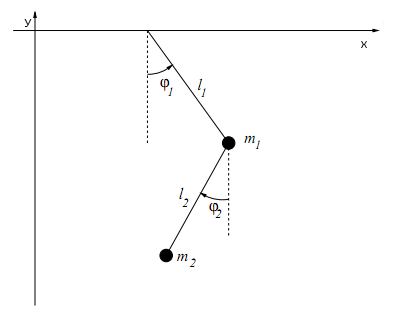
\includegraphics[scale=0.8]{doppelpendel.png}
	\caption{Doppelpendel mit wichtigen Größen \protect\footnotemark}
\end{figure}
\footnotetext{Quelle: http://me-lrt.de/img/vari-u05-2-doppelpendel.png}

Man kann es mit folgendem System gekoppelter Differentialgleichungen beschreiben.
\begin{align}
	Ml_1\ddot{\varphi}_1 + m_2l_2\ddot{\varphi}_2\cos\left(\varphi_1-\varphi_2\right) + m_2l_2\dot{\varphi}_2^2\sin\left(\varphi_1-\varphi_2\right) + Mg\sin\varphi_1 &= 0 \label{eq:bew1} \\
	m_2l_2\ddot{\varphi}_2 + m_2l_1\ddot{\varphi}_1\cos\left(\varphi_1-\varphi_2\right) - m_2l_1\dot{\varphi}_1^2\sin\left(\varphi_1-\varphi_2\right) + m_2g\sin\varphi_2&=0 \label{eq:bew2}
\end{align}
Dabei ist $M=m_1+m_2$.
Zuerst soll dieses System 2.Ordnung auf eines erster Ordnung zurückgeführt werden, um diese anschließend mittels Runge-Kutta-Verfahren 2. und 4.Ordnung numerisch zu integrieren.\\
Man fixiert $l_1=1\si{\meter}$ und $m_1=1\si{\kilo\gram}$ und variiert die Verhältnisse $l_2/l_1$ und $m_2/m_1$.
Für die Anfangsbedingungen $\varphi_1(0)=\frac{\pi}{4}$, $\dot{\varphi}_1=1 \frac{\si{rad}}{\si{\second}}$ und $\varphi_2(0)=\frac{\pi}{3}$, $\dot{\varphi}_2=1.5 \frac{\si{rad}}{\si{\second}}$ wird dann das Verhalten des Pendels untersucht.
Es soll die Bahn der beiden Massen geplottet werden sowie ihre Geschwindigkeiten in Abhängigkeit des Ortes.
Neben dem qualitativen Verhalten des Pendels sollen auch die beiden genutzten Integrationsverfahren hinsichtlich Geschwindigkeit und Genauigkeit getestet werden.

\section{System umschreiben}
Stellt man \eqref{eq:bew2} nach $\ddot{\varphi}_2$ um und setzt man dies in \eqref{eq:bew1} ein, kann diese Gleichung nach $\ddot{\varphi}_1$ aufgelöst werden. Analog stellt man \eqref{eq:bew2} nach $\ddot{\varphi}_1$ um und setzt dies in \eqref{eq:bew1} ein, um $\ddot{\varphi}_2$ zu erhalten. 
\begin{align}
	\ddot{\varphi}_1 &= -\left(m_2l_1\dot{\varphi}_1^2sc - m_2g\sin\varphi_2c + m_2l_2\dot{\varphi}_2^2s+Mg\sin\varphi_1 \right)/ \left(l_1M-l_1m_2c^2\right)\\
	\ddot{\varphi}_2 &= \left(Ml_1\dot{\varphi}_1^2s - Mg\sin\varphi_2 + m_2l_2\dot{\varphi}_2^2sc+Mg\sin\varphi_1c \right)/ \left(l_2M-l_2m_2c^2\right)
\end{align}
Hier ist $s=\sin\left(\varphi_1-\varphi_2\right)$ und $c=\cos\left(\varphi_1-\varphi_2\right)$.\\
Nun hängen die zweiten Ableitungen nicht mehr von der jeweils anderen zweiten Ableitung ab.
Substituiert man nun noch $\dot{\varphi}_1$ bsp. durch $\theta_1$ und analog $\dot{\varphi}_2$ durch $\theta_2$, sind diese 4 Gleichungen ein System erster Ordnung.
Dies kann nun numerisch gelöst werden. 

\section{Kartesische Koordinaten und Energie}
Aus den Winkeln und Seillängen lassen sich so die kartesischen Koordinaten berechnen:
\begin{align*}
	x_1 &= l_1\sin\varphi_1\\
	y_1 &= -l_1\cos\varphi_1\\	
	x_2 &= x_1+l_2\sin\varphi_2\\
	y_2 &= y_1-l_2\cos\varphi_2\\
\end{align*}
Leitet man diese ab, erhält man die Geschwindigkeiten.
\begin{align*}
	\dot{x}_1 &= l_1\cos\varphi_1 \cdot \dot{\varphi}_1\\
	\dot{y}_1 &= l_1\sin\varphi_1 \cdot \dot{\varphi}_1\\	
	\dot{x}_2 &= \dot{x}_1 + l_2\cos\varphi_2 \cdot \dot{\varphi}_2\\
	\dot{y}_2 &= \dot{y}_1 + l_2\sin\varphi_2 \cdot \dot{\varphi}_2\\
\end{align*}
Aus all diesen Werten kann die Gesamtenergie des Doppelpendels berechnet werden:
\begin{align*}
	E = E_{pot}+E_{kin} = m_1gy_1+m_2gy_2 + \frac{1}{2}m_1\left(\dot{x}_1^2+\dot{y}_1^2\right) + \frac{1}{2}m_2\left(\dot{x}_2^2+\dot{y}_2^2\right)
\end{align*}

\section{Programmaufbau}
Ich habe mich für den objektorientierten Ansatz entschieden.
So beschreibt die Klasse \textit{Doppelpendel} eben dieses. 
Sie hat folgende Attribute:
\begin{itemize}
	\item Massen und Längen	
	\item $\varphi_1$ und $\varphi_2$ sowie ihre ersten Ableitungen
	\item zugehörige kartesische Koordinaten - auch Geschwindigkeiten
	\item Energie - anfangs und aktuell
	\item Saltozähler
	\item Zeit
\end{itemize}
Die Berechnung der Energie dient der Beurteilung, wie gut die Trajektorie berechnet wurde, da sie konstant sein sollte.
Die Zählung der Saltos - also wenn die Winkel $82n+1)\pi$ überschreiten - habe ich hinzugefügt, um das Verhalten des Pendels einfacher beurteilen zu können, vor allem in Hinblick auf verschiedene Massen- und Längenverhältnisse.
So muss nicht jede Trajektorie angeschaut werden.\\
Der \textit{Konstruktor} setzt $m_1=1\si{\kilo\gram}$ und $l_1=1\si{\meter}$, da wir uns hier nur auf diesen Fall beschränken.
Da alle Attribute jedoch \textit{public} sind, könnte man diese beiden auch ändern.
Mit der Memberfunktion \textit{initialize} werden die restlichen Variablen gesetzt.
So kann diese öfters aufgerufen werden und das Doppelpendel mit neuen Anfangsbedingungen gestartet werden.\\
Berechnung der Trajektorie\\
Außerdem hat sie noch weitere Methoden:
\begin{itemize}
	\item $\ddot{\varphi}_1\left(\varphi_1, \dot{\varphi}_1,\varphi_2, \dot{\varphi}_2\right)$ und $\ddot{\varphi}_2\left(\varphi_1, \dot{\varphi}_1,\varphi_2, \dot{\varphi}_2\right)$
	\item Runge-Kutta 2. und 4.Ordnung
	\item Berechnung der kartesischen Koordinaten und deren Ableitungen
	\item Berechnung der Gesamtenergie
\end{itemize}

Des Weiteren habe ich noch zwei Methoden implementiert, die den Abstand der Massen zwei verschiedener Doppelpendel zurückgibt.
Diese werden in den Methoden \textit{rk2VSrk4} und \textit{variiereVerhaeltnisseQuantitativ} genutzt, um die beiden Trajektorien zu vergleichen, die durch die benutzen Integrationsverfahren entstehen.
Während die zuerst genannte Funktion das zeitliche Verhalten eines bestimmten Doppelpendels berechnet, untersucht die zweite das allgemeine Verhalten bei verschiedenen Längen-/Massenverhältnissen nach den von mir eingeführten Parametern, also Energie, Zahl der Überschläge und Summe der Abstände.
Dies soll mir später helfen, interessante Konstellationen leichter zu finden.

\section{Auswertung}
\subsection{Scan}
Variiert man Längen- und Massenverhältnisse und beobachtet dabei die Zahl der Überschläge (siehe Anhang -> Scan), erkennt man Bereiche, in denen gar keine Überschäge stattfinden. Man erwartet eher "langweilige" Trajektorien. An Stellen mit hohen Überschlagsraten kann men interessantere Bahnen erwarten.
Vergleicht man jedoch noch die Energie, die das Doppelpendel am Ende der Simulation mit der Anfangsenergie, stellt man fest, dass die Energie auch an den interessanten Stellen ungewöhnlich zugenommen hat.
So kann man den Daten nicht ganz trauen.

\subsection{Trajektorien}
Hier sind ein paar Trajektorien der zweiten Masse dargestellt, die die verschiedenen Verhaltensweisen des Pendels darstellen sollen. Von langsamen Hin-und-Her-Schwingen bis wirren Bewegungen ist alles dabei.
Auf das Darstellen der ersten Masse habe ich verzichtet, da sie sich nur auf einer Kreisbahn bewegen kann.

\begin{figure}[!htb]
	\centering
	\subfigure[$l_2=5.75\si{\meter}$, $m_2=7\si{\kilo\gram}$, 20 Sekunden, $\Delta t = 0.005 \si{\second}$]
	  {\begin{adjustbox}{width=0.43\linewidth}\subimport*{Programm/}{trajektorie1.tex}\end{adjustbox}}
	  \hfill
	  \subfigure[$l_2=0.5\si{\meter}$, $m_2=0.05\si{\kilo\gram}$, 20 Sekunden, $\Delta t = 0.005 \si{\second}$]
	  {\begin{adjustbox}{width=0.43\linewidth}\subimport*{Programm/}{trajektorie2.tex}\end{adjustbox}}
	  \hfill
	  \subfigure[$l_2=1\si{\meter}$, $m_2=1\si{\kilo\gram}$, 20 Sekunden, $\Delta t = 0.005 \si{\second}$]
	  {\begin{adjustbox}{width=0.43\linewidth}\subimport*{Programm/}{trajektorie3.tex}\end{adjustbox}}
	\caption{verschiedene Trajektorien der zweiten Masse}
\end{figure}

\begin{figure}[!htb]
	\centering
	\subfigure[$l_2=3\si{\meter}$, $m_2=0.6\si{\kilo\gram}$, 20 Sekunden, $\Delta t = 0.005 \si{\second}$]
	  {\begin{adjustbox}{width=0.43\linewidth}\subimport*{Programm/}{trajektorie4.tex}\end{adjustbox}}
	  \hfill
	  \subfigure[$l_2=3\si{\meter}$, $m_2=0.6\si{\kilo\gram}$, 40 Sekunden, $\Delta t = 0.005 \si{\second}$]
	  {\begin{adjustbox}{width=0.43\linewidth}\subimport*{Programm/}{trajektorie5.tex}\end{adjustbox}}
	\caption{Trajektorie der zweiten Masse - Zeitdauer verschieden}
\end{figure}

\subsection{Geschwindigkeiten}
Unter Anhang->Geschwindigkeiten habe ich zur ersten Konstellation die Geschwindigkeiten aufgetragen. Zu jeder kartesischen Koordinate wird die Geschwindigkeit entlang dieser und der anderen Achse aufgetragen.
Dies wir für beide Massen gemacht.
Ein 3D-Plot ist nicht sinnvoll, da man dort nichts erkennen konnte.\\
Man sieht die Unterschiede der beiden Integrationsverfahren.
Merkwürdigerweise sind die erreichten Geschwindigkeiten beim Runge-Kutta-Verfahren 4.Ordnung zum Teil viel größer als die mit dem 2.Ordnung.
Dies soll später genauer untersucht werden.

\subsection{Entwicklung der Gesamtenergie}
Um die Genauigkeit des Integrationsverfahrens zu überprüfen, kann man sich die Gesamtenergie anschauen.
Diese sollte bekanntlich konstant sein.
Zu den obigen Trajektorien ist diese Entwicklung unter Anhang -> Kontrollstrukturen zu finden.
Man erkennt Spitzen, danach pendelt sie sich wieder auf dem gleich Niveau ein.
Simuliert man jedoch über längere Zeiten ist dies nicht der Fall und sie steigt und steigt. Die Simulation ist also wertlos.

\subsection{Vergleich der Integrationsverfahren}
Zwar ist Runge-Kutta 2.Ordnung mit gleicher Integrationsschrittweite schneller als der 4.Ordnung, aber allgemein auch ungenauer. 
Dies ist bei einem chaotischen System wie diesem unerwünscht.\\
Vergleicht man jedoch die Entwicklung der Gesamtenergie, stellt man fest, dass auf unerklärliche Weise die Energie in Abb. 10 bei dem Verfahren 4.Ordnung steigt und sich letztlich auf einem höheren Niveau einpendelt, als bei dem Verfahren 2.Ordnung.
Dies scheint jedoch nur Zufall zu sein, denn allgemein - wie in Abb 14 zu sehen, ist das Verfahren 4.Ordnung genauer sein.\\ 
Da wir hier ein chaotisches System vorliegen haben, ist es sinnvoll, nur eine kurze Zeitspanne zu simulieren, da kleinste Abweichungen von der richtigen Bahn große Auswirkungen haben.

\section{Anhang}
\subsection{Scan}
\begin{figure}[!htb]
	\centering
	\subimport*{Programm/}{salto1rk4.tex}
	\caption{Zahl der Überschläge der ersten Masse nach 20 Sekunden mitttels Runge-Kutta 4.Ordnung}
\end{figure}

\begin{figure}[!htb]
	\centering
	\subimport*{Programm/}{salto2rk4.tex}
	\caption{Zahl der Überschläge der zweiten Masse nach 20 Sekunden mitttels Runge-Kutta 4.Ordnung}
\end{figure}

\begin{figure}[!htb]
	\centering
	\subimport*{Programm/}{energie_rk4.tex}
	\caption{Energie nach 20 Sekunden mitttels Runge-Kutta 4.Ordnung}
\end{figure}

\begin{figure}[!htb]
	\centering
	\subimport*{Programm/}{energie0_rk4.tex}
	\caption{Anfangsenergie}
\end{figure}
\newpage
\subsection{Geschwindigkeiten}
\begin{figure}
	\centering
	\subfigure[$x_1:\dot{x}_1$]
	  {\begin{adjustbox}{width=0.43\linewidth}\subimport*{Programm/}{geschw1_xvx1.tex}\end{adjustbox}}
	  \hfill
	\subfigure[$x_1:\dot{y}_1$]
	  {\begin{adjustbox}{width=0.43\linewidth}\subimport*{Programm/}{geschw1_xvy1.tex}\end{adjustbox}}
	  \hfill
	\subfigure[$y_1:\dot{x}_1$]
	  {\begin{adjustbox}{width=0.43\linewidth}\subimport*{Programm/}{geschw1_yvx1}\end{adjustbox}}
	  \hfill
	\subfigure[$y_1:\dot{y}_1$]
	  {\begin{adjustbox}{width=0.43\linewidth}\subimport*{Programm/}{geschw1_yvy1}\end{adjustbox}}
  
  \caption{Geschwindigkeiten der ersten Masse bei folgenden Parametern:\\ $l_2=5.75\si{\meter}$, $m_2=7\si{\kilo\gram}$, 20 Sekunden, $\Delta t = 0.005 \si{\second}$}
  \label{fig:geschw11}
\end{figure}

\begin{figure}
	\centering
	\subfigure[$x_2:\dot{x}_2$]
	  {\begin{adjustbox}{width=0.43\linewidth}\subimport*{Programm/}{geschw1_xvx2.tex}\end{adjustbox}}
	  \hfill
	\subfigure[$x_2:\dot{y}_2$]
	  {\begin{adjustbox}{width=0.43\linewidth}\subimport*{Programm/}{geschw1_xvy2.tex}\end{adjustbox}}
	  \hfill
	\subfigure[$y_2:\dot{x}_2$]
	  {\begin{adjustbox}{width=0.43\linewidth}\subimport*{Programm/}{geschw1_yvx2}\end{adjustbox}}
	  \hfill
	\subfigure[$y_2:\dot{y}_2$]
	  {\begin{adjustbox}{width=0.43\linewidth}\subimport*{Programm/}{geschw1_yvy2}\end{adjustbox}}
  
  \caption{Geschwindigkeiten der ersten Masse bei folgenden Parametern:\\ $l_2=5.75\si{\meter}$, $m_2=7\si{\kilo\gram}$, 20 Sekunden, $\Delta t = 0.005 \si{\second}$}
  \label{fig:geschw12}
\end{figure}

\newpage
\subsection{Kontrollstrukturen}
\begin{figure}
	\centering
	\subfigure[Energie]
	  {\begin{adjustbox}{width=0.43\linewidth}\subimport*{Programm/}{energie1.tex}\end{adjustbox}}
	  \hfill
	\subfigure[Summe der Abstände]
	  {\begin{adjustbox}{width=0.43\linewidth}\subimport*{Programm/}{dsum1.tex}\end{adjustbox}}
  
  \caption{$l_2=5.75\si{\meter}$, $m_2=7\si{\kilo\gram}$, 20 Sekunden, $\Delta t = 0.005 \si{\second}$}
  \label{fig:geschw12}
\end{figure}

\begin{figure}
	\centering
	\subfigure[Energie]
	  {\begin{adjustbox}{width=0.43\linewidth}\subimport*{Programm/}{energie2.tex}\end{adjustbox}}
	  \hfill
	\subfigure[Summe der Abstände]
	  {\begin{adjustbox}{width=0.43\linewidth}\subimport*{Programm/}{dsum2.tex}\end{adjustbox}}
  
  \caption{$l_2=0.5\si{\meter}$, $m_2=0.05\si{\kilo\gram}$, 20 Sekunden, $\Delta t = 0.005 \si{\second}$}
  \label{fig:geschw12}
\end{figure}


\begin{figure}
	\centering
	\subfigure[Energie]
	  {\begin{adjustbox}{width=0.43\linewidth}\subimport*{Programm/}{energie3.tex}\end{adjustbox}}
	  \hfill
	\subfigure[Summe der Abstände]
	  {\begin{adjustbox}{width=0.43\linewidth}\subimport*{Programm/}{dsum3.tex}\end{adjustbox}}
  
  \caption{$l_2=1\si{\meter}$, $m_2=1\si{\kilo\gram}$, 20 Sekunden, $\Delta t = 0.005 \si{\second}$}
  \label{fig:geschw12}
\end{figure}


\begin{figure}
	\centering
	\subfigure[Energie]
	  {\begin{adjustbox}{width=0.43\linewidth}\subimport*{Programm/}{energie4.tex}\end{adjustbox}}
	  \hfill
	\subfigure[Summe der Abstände]
	  {\begin{adjustbox}{width=0.43\linewidth}\subimport*{Programm/}{dsum4.tex}\end{adjustbox}}
  
  \caption{$l_2=3\si{\meter}$, $m_2=0.6\si{\kilo\gram}$, 20 Sekunden, $\Delta t = 0.005 \si{\second}$}
  \label{fig:geschw12}
\end{figure}


\begin{figure}
	\centering
	\subfigure[Energie]
	  {\begin{adjustbox}{width=0.43\linewidth}\subimport*{Programm/}{energie5.tex}\end{adjustbox}}
	  \hfill
	\subfigure[Summe der Abstände]
	  {\begin{adjustbox}{width=0.43\linewidth}\subimport*{Programm/}{dsum5.tex}\end{adjustbox}}
  
  \caption{$l_2=3\si{\meter}$, $m_2=0.6\si{\kilo\gram}$, 40 Sekunden, $\Delta t = 0.005 \si{\second}$}
  \label{fig:geschw12}
\end{figure}

\end{document}
